\section{Preparación del kit}
\subsection{Creación o asignación de un titular}
La plataforma Azure Sphere es muy estricta con el uso de sus microcontroladores, por lo que antes de desarrollar en ella tenemos que hacer un procedimiento para tenerla lista. Esta plataforma utiliza algo llamado inquilinos (tenants en inglés), que son la forma en que se organizan los permisos a la hora de desarrollar en el kit, en este inquilino, múltiples usuarios pueden estar conectados para desarrollar en las tarjetas que estén registradas. Cada microcontrolador solo puede conectarse a un inquilino, por lo que se necesita ser muy cuidadoso a la hora de registrarlo.

\begin{figure}[h]
	\centering
	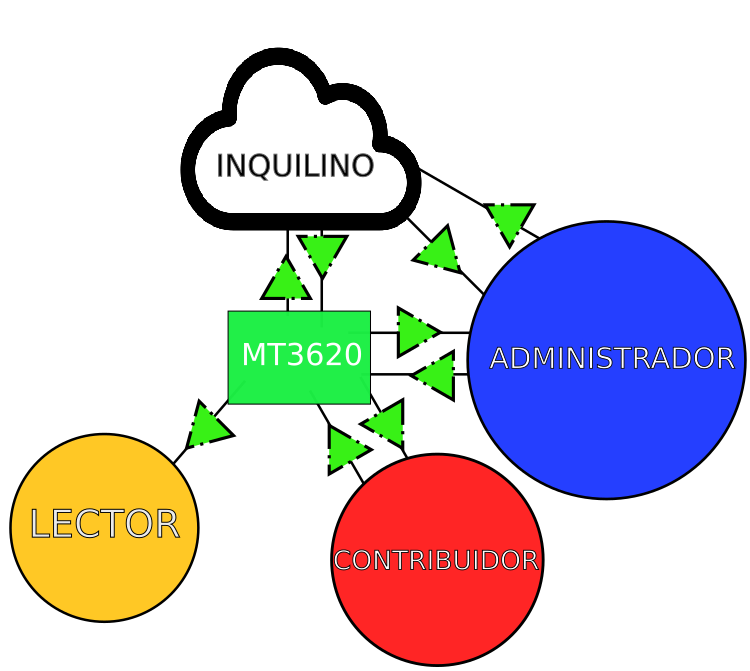
\includegraphics[scale = 1.25]{tenant}
	\caption{Organización de desarrollo.}
\end{figure}

Primero, en la terminal de tu sistema operativo, deberás de registrar un correo (que use los servicios de Microsoft) a la plataforma: 
\begin{verbatim}
	azshpere register-user --new-user <correo-electronico>
\end{verbatim}

Inicia sesión con el siguiente comando:
\begin{verbatim}
	azsphere login
\end{verbatim}

\subsubsection{Registro del dispositivo}
\textit{Tener en cuenta que esta operación NO se pude revertir.}
\linebreak
\linebreak
Primero necesitas tener el dispositivo conectado a tu ordenador. Después se necesita ver si tu cuenta no tiene algún inquilino disponible; esto se hace con el comando:
\begin{verbatim}
	azsphere tenant list
\end{verbatim}
Si aparecen uno o varios inquilinos, solo sería seleccionar uno con el comando:
\begin{verbatim}
	azsphere tenant select --tenant <nombre o ID del tenant>
\end{verbatim}

En el caso de que no salga ninguno, tienes dos opciones: pides al administrador de un inquilino que agregue tu cuenta y te dé un rol con los siguientes comandos:
\begin{verbatim}
azsphere register-user --new-user <correo-electronico>
azsphere role add --role <rol> --user <correo-electronico>
\end{verbatim}
O se crea un inquilino:
\begin{verbatim}
	azsphere tenant create --name <nombre-del-tenant>
\end{verbatim}
Al crear un nuevo inquilino, tu usuario tendrá el rol de administrador por defecto.


\subsubsection{Roles en un inquilino}
\begin{itemize}
	\item 
	Administrador: tiene acceso completo a todos los dispositivos y operaciones, también puede añadir o eliminar a otros usuarios. Se recomienda solo dos cuentas con este rol.
	\item 
	Contribuidor: Pueden registrar dispositivos, hacer cambios o implementaciones, pero no eliminar operaciones. Básicamente, pueden hacer desarrollo en el kit, pero no administrar el inquilino.
	\item 
	Lector: Tiene la capacidad de leer la información del inquilino, los dispositivos registrados, implementaciones y errores. Este rol es apropiado para el mantenimiento.
	
\end{itemize}

\subsection{Conectando el MT3620 a Internet}
Se tiene que conectar el microcontrolador a una red de internet para que pueda recibir actualizaciones y pueda comunicarse al centro de IoT de Azure. Esto se hace a partir de la IDE que estés usando.
Si quieres comprobar primero que tu microcontrolador este conectado a internet utiliza:

\begin{verbatim}
	azsphere device wifi show-status
\end{verbatim}

\subsubsection{Visual Studio}
\begin{itemize}
	\item
	Conectas la Azure Sphere a tu computadora.
	\item 
	En el menú selecciona Ver $\rightarrow$ Otra Ventana $\rightarrow$ Explorador de Azure Sphere.
	(View $\rightarrow$ Other Windows $\rightarrow$ Azure Sphere Explorer)
	
	\begin{figure}[h]
		\centering
		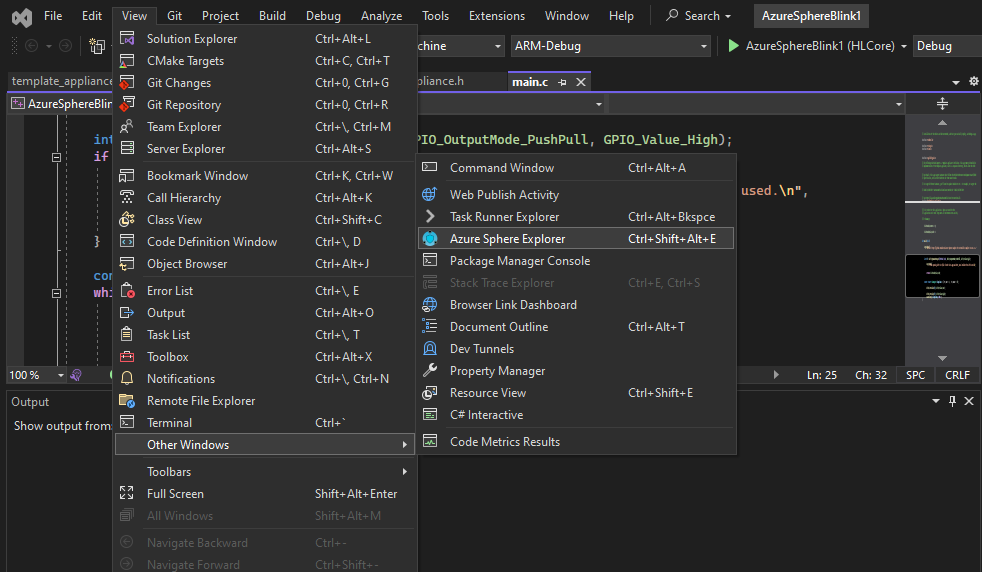
\includegraphics[width=0.75\textwidth,height=\textheight,keepaspectratio]{VS2}
		\caption{Menú de la pestaña.}
	\end{figure}

	\pagebreak
	\item 
	Desglosa el dispositivo del menú. 
	\begin{figure}[h]
		\centering
		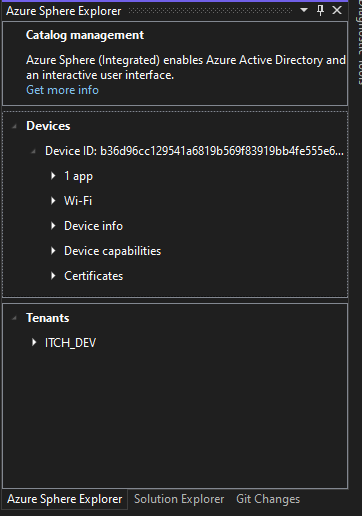
\includegraphics[width=0.65\textwidth,height=\textheight,keepaspectratio]{VS3}
		\caption{Menú del dispositivo.}
	\end{figure}

	\pagebreak
	\item 
	Expande la sección de Wi-Fi.

	\begin{figure}[h]
		\centering
		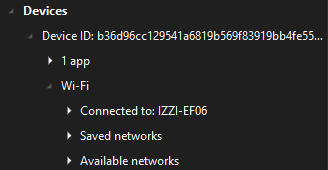
\includegraphics[width=\textwidth,height=\textheight,keepaspectratio]{VS4}
		\caption{Sección de Wi-Fi del menú.}
	\end{figure}

	\item 
	Si en uno de los elementos te indica como desconectado, entonces expande la sección de redes disponibles.
	\item 
	Selecciona la red que deseas e ingresa la contraseña.
\end{itemize}
\pagebreak
\subsubsection{Visual Studio Code}
\begin{itemize}
	\item
	Conectas la Azure Sphere a tu computadora.
	\item 
	Presiona el botón de Ver $\rightarrow$ Abrir Vista... . (View $\rightarrow$ Open View...)
	\begin{figure}[h]
	\centering
	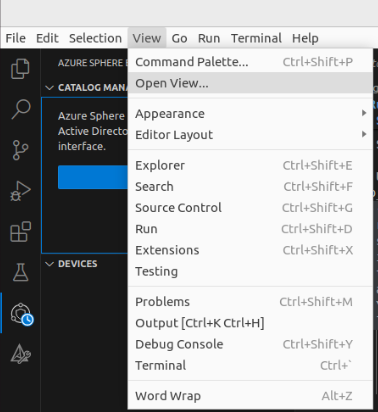
\includegraphics[width=0.75\textwidth,height=\textheight,keepaspectratio]{VSCode2}
	\caption{Menú de la pestaña.}
	\end{figure}
	\item 
	Escriba la palabra Azure y seleccione Azure Sphere Explorer; aparecerá un menú en la sección lateral del VSCode.  
	\begin{figure}[h]
	\centering
	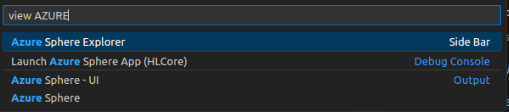
\includegraphics[width=0.75\textwidth,height=\textheight,keepaspectratio]{VSCode2-5}
	\caption{Ventana de comandos.}
	\end{figure}
	\pagebreak
	\item 
	Desglosa el dispositivo del menú. 
	\begin{figure}[h]
	\centering
	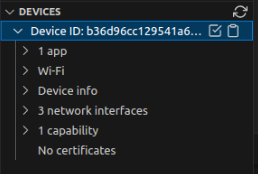
\includegraphics[width=.75\textwidth,height=\textheight,keepaspectratio]{VSCode3}
	\caption{Menú del dispositivo.}
	\end{figure}
	\item 
	Expande la sección de Wi-Fi.
	\begin{figure}[h]
	\centering
	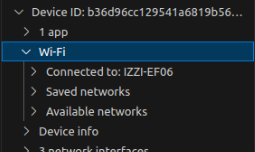
\includegraphics[width=0.75\textwidth,height=\textheight,keepaspectratio]{VSCode4}
	\caption{Sección de Wi-Fi del menú.}
	\end{figure}
	\item 
	Si en uno de los elementos te indica como desconectado, entonces expande la sección de redes disponibles.
	\item 
	Selecciona la red que deseas e ingresa la contraseña.
\end{itemize}

\subsection{Habilitar desarrollo del microcontrolador}
Por último tienes que habilitar el modo desarrollador para poder grabar algo en el MCU. Esto se hace desde la terminal con el siguiente comando:
\begin{verbatim}
azsphere device enable-development
\end{verbatim}

%\subsection{Compilar y cargar un programa al MC}
%En el editor, primero cargar un proyecto cualquiera, puede ser uno de los que provee el SDK.
